% Note that the a4paper option is mainly intended so that authors in
% countries using A4 can easily print to A4 and see how their papers will
% look in print. Authors are encouraged to use U.S. letter paper when 
% submitting to IEEE. Use the testflow package mentioned above to verify
% correct handling of both paper sizes by the author's LaTeX system.
%
% Also note that the "draftcls" or "draftclsnofoot", not "draft", option
% should be used if it is desired that the figures are to be displayed in
% draft mode.
%
% This paper can be formatted using the peerreviewca
% (instead of conference) mode.
\documentclass[conference, a4paper]{IEEEtran}
% If the IEEEtran.cls has not been installed into the LaTeX system files, 
% manually specify the path to it:
% \documentclass[conference]{../sty/IEEEtran} 


% some very useful LaTeX packages include:
\usepackage{cite}      % Written by Donald Arseneau
                        % V1.6 and later of IEEEtran pre-defines the format
                        % of the cite.sty package \cite{} output to follow
                        % that of IEEE. Loading the cite package will
                        % result in citation numbers being automatically
                        % sorted and properly "ranged". i.e.,
                        % [1], [9], [2], [7], [5], [6]
                        % (without using cite.sty)
                        % will become:
                        % [1], [2], [5]--[7], [9] (using cite.sty)
                        % cite.sty's \cite will automatically add leading
                        % space, if needed. Use cite.sty's noadjust option
                        % (cite.sty V3.8 and later) if you want to turn this
                        % off. cite.sty is already installed on most LaTeX
                        % systems. The latest version can be obtained at:
                        % http://www.ctan.org/tex-archive/macros/latex/contrib/supported/cite/

%\usepackage{graphicx}  % Written by David Carlisle and Sebastian Rahtz
                        % Required if you want graphics, photos, etc.
                        % graphicx.sty is already installed on most LaTeX
                        % systems. The latest version and documentation can
                        % be obtained at:
                        % http://www.ctan.org/tex-archive/macros/latex/required/graphics/
                        % Another good source of documentation is "Using
                        % Imported Graphics in LaTeX2e" by Keith Reckdahl
                        % which can be found as esplatex.ps and epslatex.pdf
                        % at: http://www.ctan.org/tex-archive/info/
% NOTE: for dual use with latex and pdflatex, instead load graphicx like:
\ifx\pdfoutput\undefined
\usepackage[dvipdfm]{graphicx}
\else
\usepackage[pdftex]{graphicx}
\fi

% However, be warned that pdflatex will require graphics to be in PDF
% (not EPS) format and will preclude the use of PostScript based LaTeX
% packages such as psfrag.sty and pstricks.sty. IEEE conferences typically
% allow PDF graphics (and hence pdfLaTeX). However, IEEE journals do not
% (yet) allow image formats other than EPS or TIFF. Therefore, authors of
% journal papers should use traditional LaTeX with EPS graphics.
%
% The path(s) to the graphics files can also be declared: e.g.,
% \graphicspath{{../eps/}{../ps/}}
% if the graphics files are not located in the same directory as the
% .tex file. This can be done in each branch of the conditional above
% (after graphicx is loaded) to handle the EPS and PDF cases separately.
% In this way, full path information will not have to be specified in
% each \includegraphics command.
%
% Note that, when switching from latex to pdflatex and vice-versa, the new
% compiler will have to be run twice to clear some warnings.


%\usepackage{psfrag}    % Written by Craig Barratt, Michael C. Grant,
                        % and David Carlisle
                        % This package allows you to substitute LaTeX
                        % commands for text in imported EPS graphic files.
                        % In this way, LaTeX symbols can be placed into
                        % graphics that have been generated by other
                        % applications. You must use latex->dvips->ps2pdf
                        % workflow (not direct pdf output from pdflatex) if
                        % you wish to use this capability because it works
                        % via some PostScript tricks. Alternatively, the
                        % graphics could be processed as separate files via
                        % psfrag and dvips, then converted to PDF for
                        % inclusion in the main file which uses pdflatex.
                        % Docs are in "The PSfrag System" by Michael C. Grant
                        % and David Carlisle. There is also some information 
                        % about using psfrag in "Using Imported Graphics in
                        % LaTeX2e" by Keith Reckdahl which documents the
                        % graphicx package (see above). The psfrag package
                        % and documentation can be obtained at:
                        % http://www.ctan.org/tex-archive/macros/latex/contrib/supported/psfrag/

\usepackage{subfigure} % Written by Steven Douglas Cochran
                        % This package makes it easy to put subfigures
                        % in your figures. i.e., "figure 1a and 1b"
                        % Docs are in "Using Imported Graphics in LaTeX2e"
                        % by Keith Reckdahl which also documents the graphicx
                        % package (see above). subfigure.sty is already
                        % installed on most LaTeX systems. The latest version
                        % and documentation can be obtained at:
                        % http://www.ctan.org/tex-archive/macros/latex/contrib/supported/subfigure/

\usepackage{url}       % Written by Donald Arseneau
                        % Provides better support for handling and breaking
                        % URLs. url.sty is already installed on most LaTeX
                        % systems. The latest version can be obtained at:
                        % http://www.ctan.org/tex-archive/macros/latex/contrib/other/misc/
                        % Read the url.sty source comments for usage information.

%\usepackage{stfloats}  % Written by Sigitas Tolusis
                        % Gives LaTeX2e the ability to do double column
                        % floats at the bottom of the page as well as the top.
                        % (e.g., "\begin{figure*}[!b]" is not normally
                        % possible in LaTeX2e). This is an invasive package
                        % which rewrites many portions of the LaTeX2e output
                        % routines. It may not work with other packages that
                        % modify the LaTeX2e output routine and/or with other
                        % versions of LaTeX. The latest version and
                        % documentation can be obtained at:
                        % http://www.ctan.org/tex-archive/macros/latex/contrib/supported/sttools/
                        % Documentation is contained in the stfloats.sty
                        % comments as well as in the presfull.pdf file.
                        % Do not use the stfloats baselinefloat ability as
                        % IEEE does not allow \baselineskip to stretch.
                        % Authors submitting work to the IEEE should note
                        % that IEEE rarely uses double column equations and
                        % that authors should try to avoid such use.
                        % Do not be tempted to use the cuted.sty or
                        % midfloat.sty package (by the same author) as IEEE
                        % does not format its papers in such ways.

\usepackage{amsmath}   % From the American Mathematical Society
                        % A popular package that provides many helpful commands
                        % for dealing with mathematics. Note that the AMSmath
                        % package sets \interdisplaylinepenalty to 10000 thus
                        % preventing page breaks from occurring within multiline
                        % equations. Use:
\interdisplaylinepenalty=2500
                        % after loading amsmath to restore such page breaks
                        % as IEEEtran.cls normally does. amsmath.sty is already
                        % installed on most LaTeX systems. The latest version
                        % and documentation can be obtained at:
                        % http://www.ctan.org/tex-archive/macros/latex/required/amslatex/math/



% Other popular packages for formatting tables and equations include:

%\usepackage{array}
% Frank Mittelbach's and David Carlisle's array.sty which improves the
% LaTeX2e array and tabular environments to provide better appearances and
% additional user controls. array.sty is already installed on most systems.
% The latest version and documentation can be obtained at:
% http://www.ctan.org/tex-archive/macros/latex/required/tools/

% Mark Wooding's extremely powerful MDW tools, especially mdwmath.sty and
% mdwtab.sty which are used to format equations and tables, respectively.
% The MDWtools set is already installed on most LaTeX systems. The lastest
% version and documentation is available at:
% http://www.ctan.org/tex-archive/macros/latex/contrib/supported/mdwtools/


% V1.6 of IEEEtran contains the IEEEeqnarray family of commands that can
% be used to generate multiline equations as well as matrices, tables, etc.


% Also of notable interest:

% Scott Pakin's eqparbox package for creating (automatically sized) equal
% width boxes. Available:
% http://www.ctan.org/tex-archive/macros/latex/contrib/supported/eqparbox/



% Notes on hyperref:
% IEEEtran.cls attempts to be compliant with the hyperref package, written
% by Heiko Oberdiek and Sebastian Rahtz, which provides hyperlinks within
% a document as well as an index for PDF files (produced via pdflatex).
% However, it is a tad difficult to properly interface LaTeX classes and
% packages with this (necessarily) complex and invasive package. It is
% recommended that hyperref not be used for work that is to be submitted
% to the IEEE. Users who wish to use hyperref *must* ensure that their
% hyperref version is 6.72u or later *and* IEEEtran.cls is version 1.6b 
% or later. The latest version of hyperref can be obtained at:
%
% http://www.ctan.org/tex-archive/macros/latex/contrib/supported/hyperref/
%
% Also, be aware that cite.sty (as of version 3.9, 11/2001) and hyperref.sty
% (as of version 6.72t, 2002/07/25) do not work optimally together.
% To mediate the differences between these two packages, IEEEtran.cls, as
% of v1.6b, predefines a command that fools hyperref into thinking that
% the natbib package is being used - causing it not to modify the existing
% citation commands, and allowing cite.sty to operate as normal. However,
% as a result, citation numbers will not be hyperlinked. Another side effect
% of this approach is that the natbib.sty package will not properly load
% under IEEEtran.cls. However, current versions of natbib are not capable
% of compressing and sorting citation numbers in IEEE's style - so this
% should not be an issue. If, for some strange reason, the user wants to
% load natbib.sty under IEEEtran.cls, the following code must be placed
% before natbib.sty can be loaded:
%
% \makeatletter
% \let\NAT@parse\undefined
% \makeatother
%
% Hyperref should be loaded differently depending on whether pdflatex
% or traditional latex is being used:
%
\ifx\pdfoutput\undefined
\usepackage[hypertex,dvipdfm]{hyperref}
\else
\usepackage[pdftex,hypertexnames=false,pdfstartview=FitH]{hyperref}
\fi
%
% Pdflatex produces superior hyperref results and is the recommended
% compiler for such use.



% *** Do not adjust lengths that control margins, column widths, etc. ***
% *** Do not use packages that alter fonts (such as pslatex).         ***
% There should be no need to do such things with IEEEtran.cls V1.6 and later.


% correct bad hyphenation here
\hyphenation{op-tical net-works semi-conduc-tor IEEEtran}

%\usepackage[left=25mm,right=25mm,top=25mm,bottom=25mm,columnsep=9mm]{geometry}
\usepackage[thinspace,thinqspace]{SIunits}
\usepackage{multirow}
% \IEEEoverridecommandlockouts
%\renewcommand{\rmdefault}{pad}
%\renewcommand{\sfdefault}{phv}
%\renewcommand{\ttdefault}{pcr}
%\usepackage[garamond]{mathdesign}
%\usepackage[garamond]{wrisym}
\begin{document}

% paper title
\title{Parallel AWE Technique for Electrically Large Objects
Scattering}

% author names and affiliations
% use a multiple column layout for up to three different
% affiliations
% \author{\authorblockN{Michael Shell}
% \authorblockA{School of Electrical and\\Computer Engineering\\
% Georgia Institute of Technology\\
% Atlanta, Georgia 30332--0250\\
% Email: mshell@ece.gatech.edu}
% \and
% \authorblockN{Homer Simpson}
% \authorblockA{Twentieth Century Fox\\
% Springfield, USA\\
% Email: homer@thesimpsons.com}
% \and
% \authorblockN{James Kirk\\ and Montgomery Scott}
% \authorblockA{Starfleet Academy\\
% San Francisco, California 96678-2391\\
% Telephone: (800) 555--1212\\
% Fax: (888) 555--1212}}


% avoiding spaces at the end of the author lines is not a problem with
% conference papers because we don't use \thanks or \IEEEmembership


% for over three affiliations, or if they all won't fit within the width
% of the page, use this alternative format:
% 
\author{\authorblockN{Xueguan Liu, Wenfeng Cai and Huiping Guo}
\authorblockA{School of Electronics and Information Engineering\\
Soochow University, Suzhou, Jiangsu, P. R. China}
}



% use only for invited papers
%\specialpapernotice{(Invited Paper)}

% make the title area
\maketitle

\begin{abstract}
Combining AWE technique with high performance 
computing cluster systems, the parallel AWE procedure 
for EM scattering is realized with MPI. Some numerical results are presented 
to verify the proposed method. This work provides a new way to rapidly 
predict the RCS of the electrically large objects.
\end{abstract}
% \vspace{1.34ex}
\begin{keywords}
High performance computing cluster, 
parallel computation, electromagnetic scattering, AWE, RCS.
\end{keywords}

% For peer review papers, you can put extra information on the cover
% page as needed:
% \begin{center} \bfseries EDICS Category: 3-BBND \end{center}
%
% for peerreview papers, inserts a page break and creates the second title.
% Will be ignored for other modes.
\IEEEpeerreviewmaketitle



\section{Introduction}
% no \PARstart
As known, the RCS estimation and analysis of the electrically large objects 
is limited by the memory and the speed of computers. Doubtlessly, the 
parallel computation will play an important role in the EM scattering 
computation of the electrically large objects, where many scholars have paid 
their attentions to the parallel methods such as parallel FDTD, parallel 
FMM, etc., and some useful conclusions have been obtained. However, these 
methods are mainly based on the region separate method, but not the real 
parallel process using parallel system \cite{yan_yubo:analysis:2003,lu_guanghui:application:2003}. In the other hand, the 
asymptotic waveform evaluation (AWE) technique has been widely used to 
obtain rapid analysis of wideband RCS of conducting objects
\cite{reddy:fast_rcs:1998, sun_yufa:application:2002}. We 
also use the AWE technique to calculate the scattering of partially coated 
objects \cite{liu_xueguan:numerical:2004}. The purpose of this paper is to realize the rapid RCS 
estimation of the electrically large objects by using the large capability 
and high efficient of the parallel computation, and the rapidity of AWE. In section II, the RCS is formulated by combining AWE with the 
MoM with triangle-roof-top basis function, and the parallel treatment for 
computation, where the two-dimensional block-cyclic distribution
technique with MPI
is used\cite{mpi:web}, is also discussed. In section III, some numerical results of RCS 
computation are given to verify the proposed method. This work provides a 
new way to rapidly predict the RCS of the electrically large objects.

% Reminder: the "draftcls" or "draftclsnofoot", not "draft", class option
% should be used if it is desired that the figures are to be displayed while
% in draft mode.

% An example of a floating figure using the graphicx package.
% Note that \label must occur AFTER (or within) \caption.
% For figures, \caption should occur after the \includegraphics.
%
%\begin{figure}
%\centering
%\includegraphics[width=2.5in]{myfigure}
% where an .eps filename suffix will be assumed under latex, 
% and a .pdf suffix will be assumed for pdflatex
%\caption{Simulation Results}
%\label{fig_sim}
%\end{figure}


% An example of a double column floating figure using two subfigures.
%(The subfigure.sty package must be loaded for this to work.)
% The subfigure \label commands are set within each subfigure command, the
% \label for the overall fgure must come after \caption.
% \hfil must be used as a separator to get equal spacing
%
%\begin{figure*}
%\centerline{\subfigure[Case I]{\includegraphics[width=2.5in]{subfigcase1}
% where an .eps filename suffix will be assumed under latex, 
% and a .pdf suffix will be assumed for pdflatex
%\label{fig_first_case}}
%\hfil
%\subfigure[Case II]{\includegraphics[width=2.5in]{subfigcase2}
% where an .eps filename suffix will be assumed under latex, 
% and a .pdf suffix will be assumed for pdflatex
%\label{fig_second_case}}}
%\caption{Simulation results}
%\label{fig_sim}
%\end{figure*}



% An example of a floating table. Note that, for IEEE style tables, the 
% \caption command should come BEFORE the table. Table text will default to
% \footnotesize as IEEE normally uses this smaller font for tables.
% The \label must come after \caption as always.
%
%\begin{table}
%% increase table row spacing, adjust to taste
%\renewcommand{\arraystretch}{1.3}
%\caption{An Example of a Table}
%\label{table_example}
%\begin{center}
%% Some packages, such as MDW tools, offer better commands for making tables
%% than the plain LaTeX2e tabular which is used here.
%\begin{tabular}{|c||c|}
%\hline
%One & Two\\
%\hline
%Three & Four\\
%\hline
%\end{tabular}
%\end{center}
%\end{table}

\section{The Realization of the Rapid RCS Estimation}

In fact, the method discussed here for the rapid RCS estimation is suitable 
for all kinds of electrically large objects, including conducting, 
dielectric, and conducting objects coated with fully or partially material. For 
convenience, only conducting objects is considered here.

\subsection{MoM Analysis for Arbitrarily Shaped 3D Conductors}

An arbitrarily shaped 3D conductor, illuminated by a plane wave with the 
incident fields 
$(\vec{E}^\mathrm{i}, \vec{H}^\mathrm{i})$\cite{mittr73}, is shown in Fig.~\ref{fig1}, where region 0 represents for free space. The 
scattering fields $(\vec{E}^\mathrm{s}, \vec{H}^\mathrm{s})$
 in region 0 are contributed by the induced equivalent currents 
$\vec{J}$ on the surface of the conductor object. According to the boundary 
conditions, the total tangential electric fields on the perfect conductor 
surface must be zero, i.e.
\begin{equation}
\left. {\left( \vec{E}^\mathrm{i} + \vec{E}^\mathrm{s}
 \right)} \right|_{\tan } =0
\end{equation}
We use the triangle-roof-top function proposed by
Rao-Wilton-Glisson as the basis function\cite{rao_electromagnetic_scattering_by_1982}, that is
\begin{equation}
\vec{f}_n(\vec{r})=\begin{cases}
\frac{\vec{\rho}_n^{\pm}}{h_n^{\pm}}S_n^{\pm}&\vec{r}\in T_n^{\pm}\\
0&\text{others}
\end{cases}
\end{equation}
where $S_n^+ =+1,\mbox{ }S_n^- =-1$. The surface equivalent currents 
$\vec{J}$ is expanded by the basis function motioned above, then we have
\begin{equation}
\vec{J} =\sum\limits_{n=1}^N {I_n } \vec{f}_n 
\end{equation}
The incident electric fields can be expressed as
\begin{equation}
\vec{E}^\mathrm{i}=\hat {u}^\alpha E_0 
\mathrm{e}^{-\mathrm{j}\vec{k}^\mathrm{i}\cdot 
\vec{r}'}
\end{equation}
where 
$\vec{k}^\mathrm{i}$ is the incident wave vector, and $\hat {u}^\alpha $ is the 
polarization vector. Using Galerkin method, we can obtain following 
equations:
\begin{equation}
\sum\limits_{n=1}^N {Z_{mn} } I_n =V_m 
\end{equation}
Where $m=1,2,\cdots ,N$ and 
$Z_{mn} $ are the mutual impedance elements, and $V_m $ are elements 
concerned with the incident fields. 
\begin{figure}
\centerline{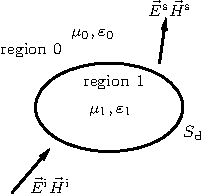
\includegraphics{fig-0}}
\caption{3D electric object.}
\label{fig1}
\end{figure}

Then we can get the expansion coefficients of equivalent currents by solving 
the above equations. We can also derive the general formula of bi-static RCS 
of arbitrarily shaped conductor objects by using the obtained expansion 
coefficients of equivalent currents as
\begin{equation}
\sigma ^\alpha =\lim\limits_{r\to \infty } 4\pi r^2\frac{\left| 
{E_\alpha^\mathrm{s}} \right|}{\left| {E^\mathrm{i}} \right|}=\frac{k^2}{4\pi }\left| 
{R^\alpha (\theta ,\phi )} \right|^2=\frac{\pi }{\lambda ^2}\left| {R^\alpha 
(\theta ,\phi )} \right|^2
\end{equation}
where $R^\alpha (\theta ,\phi )=\sum\limits_{n=1}^N {V_n \int {(\hat 
{n}^\alpha \cdot 
\vec{f} _n } 
)\mathrm{e}^{\mathrm{j}\vec{k} ^\mathrm{s}\cdot 
\vec{r}'}\mathrm{d}S_n } $.

\subsection{The Asymptotic Waveform Evaluation (AWE) Technique}

In 1998, Reddy first introduced the Pad\'{e} approach in numerical 
approach theory into the method of moments to solve EFIE \cite{reddy:fast_rcs:1998}, so the rapid 
estimation of wideband RCS was realized, and this approach is also called 
the asymptotic waveform evaluation (AWE) technique. It uses the rational 
function to decrease the computing capacity. We delivered the $n$th derivative 
of the impedance elements and excited elements used in AWE for the MoM of 
triangle-roof-top base function. These formulas are all algebraic 
expressions. They are not listed here because of their high complication. 
Using these formulas, it is convenient to rapidly estimate the wideband RCS 
of large objects through parallel treatment.

\subsection{Parallel Treatment }

For that our computation platform is a 4-node distributed-memory message-passing cluster with MPI support, the parallel treatment are emphasized to solve two problems\cite{Wilkinson:parallel:2002}, the first is 
load balance, or splitting the work reasonably evenly among the processors throughout the algorithm, the second is use of the most efficent code during computations on a single processor, to account for the memory hierarchy on each processor. To solve the first problem, we would equally 
distribute the computing task to every processor by some algorithms. To 
solve the second problem, we should do our best to use the fastest parts of 
the cluster, and decrease the communication between parts having different 
speed. In this paper, the 2D block-cyclic distribution technique with MPI is 
used to realize the above purpose\cite{blackford:slug:1997}.

The block-cyclic distribution scheme is a mapping of a set of blocks of a large matrix onto the processes. The local storage of every processor is associated 
with the large matrix by certain map relation. The precise mapping, which associates to a matrix entry identified by its global indexes the coordinates of the process that owns it and its local position within that process's memory, can be obtained by some calculation.
Every processor deals with 
the local data, so the task distribution is achieved. 
Fig.~\ref{yingshe} shows 
the mapping of a $5\times 5$ matrix partitioned into $2\times 2$ blocks mapped onto a $2\times 2$ process grid. The local entries of every matrix column are contiguously stored in the processes' memories.
\begin{figure}
\centering
\begin{tabular}{cc|cc|c}
$a_{11}$ & $a_{12}$ & $a_{13}$ & $a_{14}$ & $a_{15}$ \\
$a_{21}$ & $a_{22}$ & $a_{23}$ & $a_{24}$ & $a_{25}$ \\\hline
$a_{31}$ & $a_{32}$ & $a_{33}$ & $a_{34}$ & $a_{35}$ \\
$a_{41}$ & $a_{42}$ & $a_{43}$ & $a_{44}$ & $a_{45}$ \\\hline
$a_{51}$ & $a_{52}$ & $a_{53}$ & $a_{54}$ & $a_{55}$ \\
\multicolumn{5}{c}{\small $5\times 5$ matrix partioned in $2\times 2$
blocks}
\end{tabular}
% \hspace{2em}
\begin{tabular}{r||ccc|cc||}
 & & 0 & & \multicolumn{2}{c||}{1} \\\hline\hline
 & $a_{11}$ & $a_{12}$ & $a_{15}$ & $a_{13}$ & $a_{14}$ \\
0 & $a_{21}$ & $a_{22}$ & $a_{25}$ & $a_{23}$ & $a_{24}$ \\
 & $a_{51}$ & $a_{52}$ & $a_{55}$ & $a_{53}$ & $a_{54}$ \\\hline
\multirow{2}*{1}& $a_{31}$ & $a_{32}$ & $a_{35}$ & $a_{33}$ & $a_{34}$ \\
& $a_{41}$ & $a_{42}$ & $a_{45}$ & $a_{43}$ & $a_{44}$ \\\hline\hline
\multicolumn{6}{c}{\small $2\times 2$ process grid point of view}
\end{tabular}
\caption{A $5\times 5$ matrix decomposed into $2\times 2$ blocks mapped
onto a $2\times 2$ process grid.}\label{yingshe}
\end{figure}

In order to conveniently and efficiently use the ScaLAPACK Math
Library\cite{scalapack:web}, the 
elements derived above for AWE must be stored with the 2D block-cyclic
distribution technique. Every processor creates separately the elements to 
be locally stored. After computation by Scalapack, the scattering data will 
be sent to a main node and output to a file.

\section{Numerical Results and Discussions}

According to the principle above, we have programmed three RCS computing 
procedures of conducting object, i.e. the serial one in single frequency for 
single processor (case 1), the parallel one in single frequency for cluster 
(case 2), and the parallel one with AWE technique (case 3). As an example, a 
finite cylinder with \unit{276}{\centi\meter} length and
\unit{21.6}{\centi\meter} radius is illuminated by a plane 
wave normally to the end-surface, and the monostatic RCS in band 
\unit{330}{\mega\hertz}--\unit{440}{\mega\hertz} is calculated in three cases above. The structure and 
computation results are shown in Fig.~\ref{rslt}. The calculation results for three 
cases are almost the same, but the computing time is highly different. The 
time of case 1 for 36 frequency points is \unit{708}{\second}, the time
is \unit{341}{\second} in case 2, 
and in case 3 where the parallel AWE is used, the time for 71 frequency 
points is \unit{134}{\second}.
\begin{figure}
\centerline{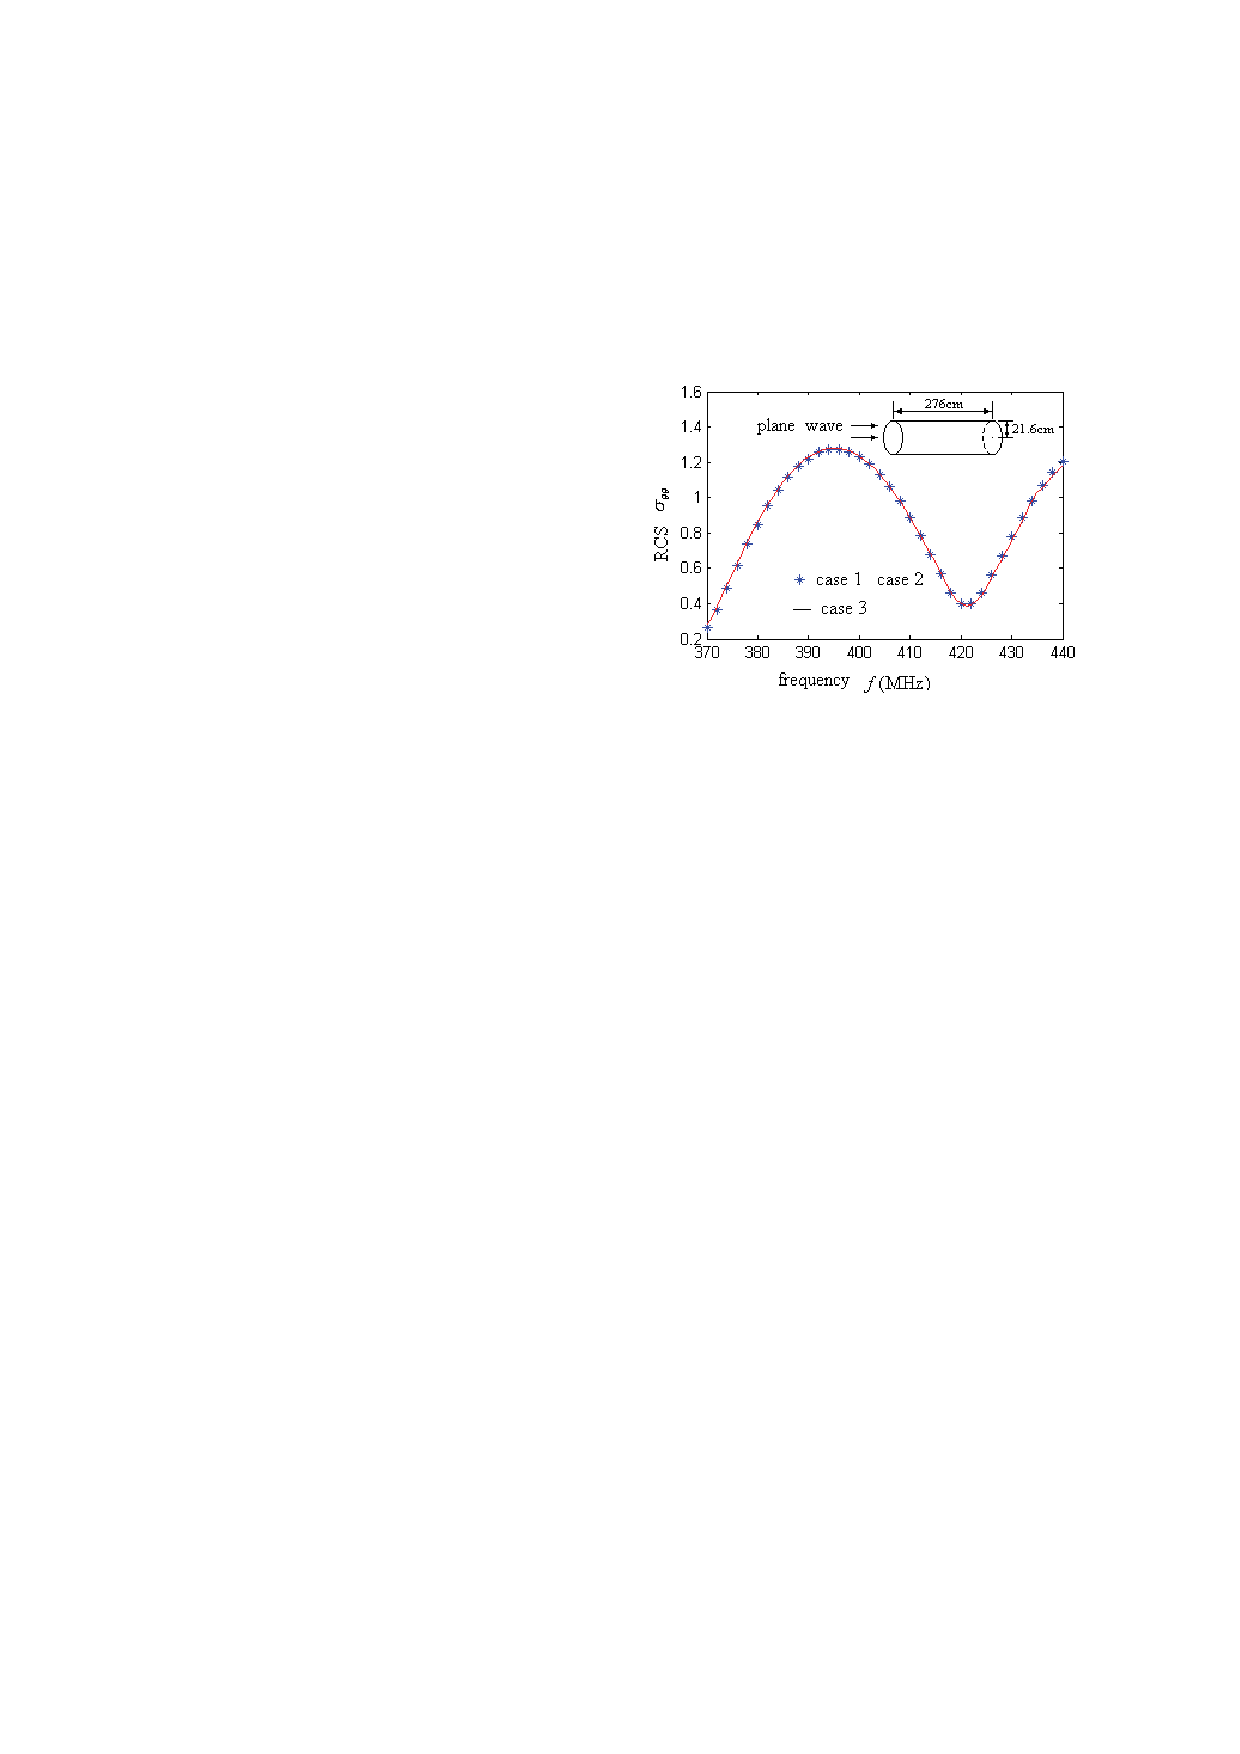
\includegraphics{pawe14}}
\caption{The computation results.}
\label{rslt}
\end{figure}

The numerical results show that the parallel computation can improve the 
computing efficient, and parallel AWE can obtained higher efficiency. In 
fact, as several equations must be solved first for parallel AWE procedure, 
so the more the calculated frequency points, the higher the efficiency to be 
achieved. In other word, for a few calculated frequency points, the parallel 
AWE is not worthy. The parallel AWE is especially suitable for wideband RCS 
estimation for large objects.

\section{Conclusion}

Parallel computation is an important trend for the computing techniques of 
electromagnetic problems, and AWE technique is suitable for rapid wideband 
RCS estimation. Combining the parallel technique and AWE technique one can 
realize rapid wideband RCS estimation for certain scale objects. But the 
method proposed here are still limited in memory size, and the computing 
time too long for more large objects. To break through these limits, the 
parallel AWE technique must be combined with other techniques (such as 
matrix sparse technique). In the other hand, for more large objects, the RCS 
changes acutely as the frequency, so the adaptive bandwidth of AWE technique 
will become less. These will be addressed in the future works of the authors.

% conference papers do not normally have an appendix

% use section* for acknowledgement
% \section*{Acknowledgment}
% optional entry into table of contents (if used)
%\addcontentsline{toc}{section}{Acknowledgment}
% The authors would like to thank...

% trigger a \newpage just before the given reference
% number - used to balance the columns on the last page
% adjust value as needed - may need to be readjusted if
% the document is modified later
 \IEEEtriggeratref{3}
% The "triggered" command can be changed if desired:
%\IEEEtriggercmd{\enlargethispage{-5in}}
%\enlargethispage{-14.6cm}
%\nocite{mittr73}
% references section
% NOTE: BibTeX documentation can be easily obtained at:
% http://www.ctan.org/tex-archive/biblio/bibtex/contrib/doc/

% can use a bibliography generated by BibTeX as a .bbl file
% standard IEEE bibliography style from:
% http://www.ctan.org/tex-archive/macros/latex/contrib/supported/IEEEtran/bibtex
\bibliographystyle{IEEEtran}
% argument is your BibTeX string definitions and bibliography database(s)
\bibliography{IEEEabrv,mybib}
%
% <OR> manually copy in the resultant .bbl file
% set second argument of \begin to the number of references
% (used to reserve space for the reference number labels box)
% that's all folks
\end{document}


